\documentclass[12pt]{article}
\usepackage{amsmath}
\usepackage{graphicx}
\usepackage{caption}
\usepackage{subcaption}
\usepackage{booktabs}
\usepackage{float}
\usepackage[utf8]{inputenc}
\usepackage{geometry}
\usepackage{multirow}
\usepackage{setspace}
\usepackage{parskip}
\usepackage{svg}
\usepackage[bottom]{footmisc}
\usepackage{tikz}
\usepackage[section]{placeins}

% This style is used to create block diagrams, you'll find it useful since many of your figures would be of that form, I'll try add more styles in the future :)
\usetikzlibrary{trees,positioning,fit,calc}
\tikzset{block/.style = {draw, fill=blue!20, rectangle,
                         minimum height=3em, minimum width=4em},
        input/.style = {coordinate},
        output/.style = {coordinate}
}

\usepackage[section]{minted}
\usepackage{xcolor}
\usemintedstyle{porland}

\usepackage{chngcntr}
\counterwithin{figure}{section}

\renewcommand{\arraystretch}{1.5}

\usepackage[hidelinks]{hyperref}
\hypersetup{
    linktoc=all
}

\renewcommand\listingscaption{Listing}
\renewcommand\listoflistingscaption{List of Listings}

\usepackage{scrhack}
\usepackage{tocbasic}
\setuptoc{lol}{levelup}

\usepackage{indentfirst}
\geometry{a4paper, margin=1in}

%------------------------------------------------%

\setlength{\parindent}{0em}
\setlength{\parskip}{0em}

\begin{document}

\begin{center}
 	{\Huge Sección 2}\\
	 \vspace{0.75cm}
	 {\large Probabilidad y Estadística ejercicios}\\
	 \vspace{0.5cm}
\end{center}
{\large Daniela Jijón, Juan Francisco Cisneros y Luciana Valdivieso}\\
\vspace{0.5cm}
{\large10 de julio de 2022}\\

\pagenumbering{Roman}
\setlength{\parskip}{\baselineskip}%

\pagenumbering{arabic}

%--------------SECCIONES ---------------------%

\section{Espacio Muestral y Probabilidad}

El espacio muestral con todas posibles combinaciones entre todas las variables que recolectamos se calculó utilizando la fórmula para combinaciones:
\begin{equation}
   C_{n}^r = \frac{n!}{(n-r)!r!}
\end{equation}

Cada observación de nuestra muestra consta de 6 variables, cuatro cuantitativas y dos categóricas. Se tiene 3 opciones para genero, 11 de edad, 10 de colegio académico, 6 año de estudio, 6 de hora de estudio y 18 opciones de GPA
\begin{equation*}
    \frac{3!}{2!1!}\cdot \frac{11!}{10!1!} \cdot\frac{10!}{9!1!} \cdot\frac{6!}{5!1!}\cdot  \frac{6!}{5!1!} \cdot \frac{18!}{17!1!}=213840
\end{equation*}
El espacio muestral contiene 213840 elementos

\section{Variables Aleatorias}
La primera variable aleatoria X muestra la diferencia entre los valores de la variable cuantitativa GPA y la media de la muestra que es 
$3.47$. 

\begin{align}
    & E(x) = \int_{-\infty}^{\infty} x\cdot f(x)dx\\
    & \begin{aligned}[t]
               V(x) &= E(x-\mu x)^{2}\\
                &= E(x^{2}) - \mu x^{2}\\
       \end{aligned}
\end{align}
Los resultados de los cálculos son:
\begin{equation*}
   E(x) = 0.026\\
\end{equation*}
\begin{equation*}
   V(x) = 0.21
\end{equation*}
La variable aleatoria sigue una distribución aproximadamente normal\\
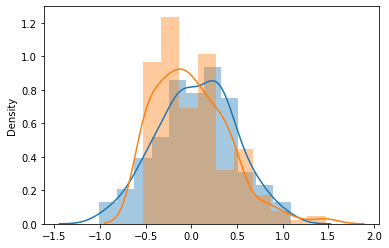
\includegraphics[width=8cm, height=7cm]{normal}

La segunda variable aleatoria Y muestra la diferencia entre los valores de la variable cuantitativa Horas de Estudio Semanales y la media de su muestra que es $12.22$\\
Se calculó la covarianza y el coeficiente de correlación entre estas dos variables aleatorias utilizando las fórmulas 4 y 5 respectivamente

\begin{align}
    & \rho xy = \frac{Cov(x,y)}{\sqrt[]{V(x)\cdot V(y)}}\\
    & \begin{aligned}[t]
	Cov(x,y) &=  E[(x-\mu x)(y-\mu y)]\\
        	&=  E(xy) - \mu x\cdot \mu \\ 
       \end{aligned}
\end{align}
Los resultados de los cálculos son:
\begin{equation*}
   Cov(x,y)= 2.69\\
\end{equation*}
\begin{equation*}
   \rho xy  = 0.79
\end{equation*}

La covarianza es positiva, lo que significa que existe una relación lineal positiva entre ambas variables. De la misma manera el coeficiente de correlación es un valor positivo considerablemente cercano a uno, lo que indica que existe una fuerte correlación entre las variables, se puede decir que entre mas horas de estudio mayor es el promedio GPA en los estudiantes.

Se seleccionaron dos variables aleatorias adicionales que describen los posibles resultados de las variables cualitativas Sexo y Colegio académico. La función de masa de probabilidad conjunta se obtuvo al calcular las frecuencias de los pares de datos en las observaciones de la muestra. 
\clearpage

La independencia de las variables aleatorias se puede comprobar multiplicando las funciones de probabilidad marginal:\\

\begin{equation}
   P(x,y)= P_{x}(x)\cdot P_{x}(y)\\
\end{equation}

Las variables son dependientes

\section{Muestreo}

Se han seleccionado dos variables aleatorias, entre ellas el GPA de los estudiantes y las horas de estudio semanales. De cada una de estas variables hemos obtenido 40 muestras aleatorias el 25\% de los datos usando Python y la función “.sample(n=50)”, para cada una de las 80 muestras se ha obtenido la media y la varianza de estas muestras graficando así las distribuciones para el GPA y las horas de estudio semanales, además de un gráfico QQ plot.\\

Los datos arrojados nos muestran que ambas distribuciones de medias y varianzas tienen una distribución normal. Esto se observa tanto visualmente debido a la forma de campana que muestra el gráfico de distribución y el gráfico QQ plot donde los datos se muestran en una línea de 45 grados.\\

Gráfico Distribución de Media para GPA y QQ Plot\\
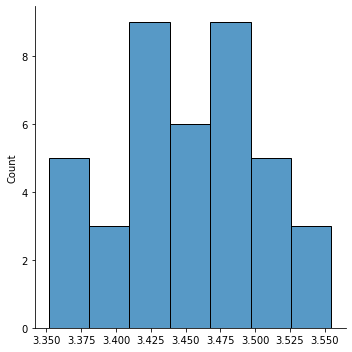
\includegraphics[width=8cm, height=7cm]{gpa_histo1}
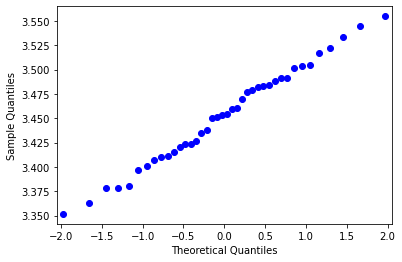
\includegraphics[width=8cm, height=7cm]{gpa_qq1}

\clearpage
Gráfico Distribución de Varianza para GPA y QQ Plot\\
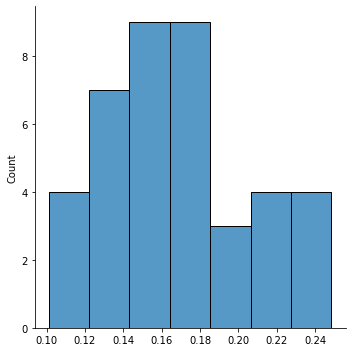
\includegraphics[width=8cm, height=7cm]{gpa_histo2}
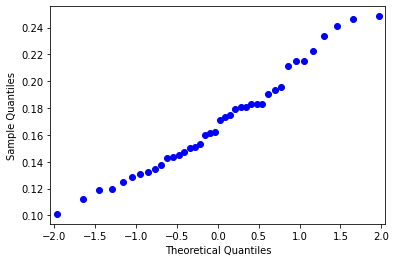
\includegraphics[width=8cm, height=7cm]{gpa_qq2}


Gráfico Distribución de Media para Horas de Estudio Semanasy QQ Plot\\
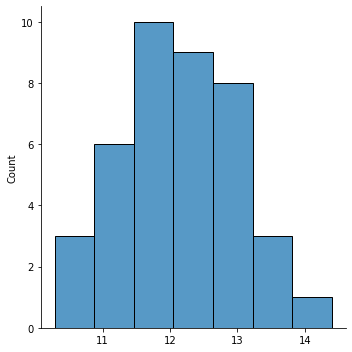
\includegraphics[width=8cm, height=7cm]{horas_histo1}
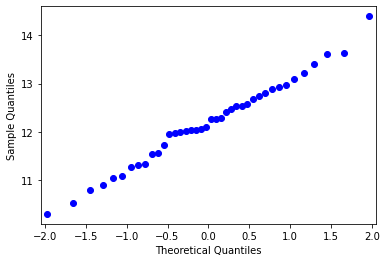
\includegraphics[width=8cm, height=7cm]{horas_qq1}

Gráfico Distribución de Varianza para Horas de Estudio Semanasy QQ Plot\\
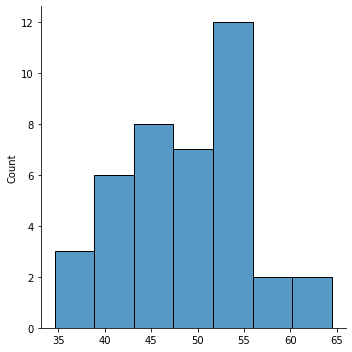
\includegraphics[width=8cm, height=7cm]{horas_histo2}
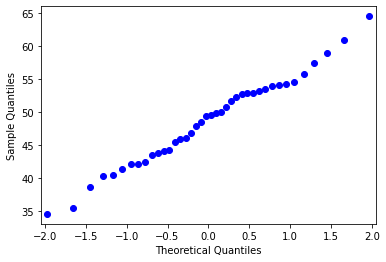
\includegraphics[width=8cm, height=7cm]{horas_qq2}

Repitiendo el ejercicio anterior pero solo obteniendo 5 muestras del 25\% de datos tanto para gpa como para horas de estudio, encontramos que los resultados ya no son distribuciones normales o por lo menos ya no se puede decir que se distribuyen de forma normal sus medias y varianzas. Esto puede ser debido a la cantidad de muestras que no es significativa para el estudio. 


Gráfico Distribución de Media para GPA y QQ Plot (5 muestras)\\
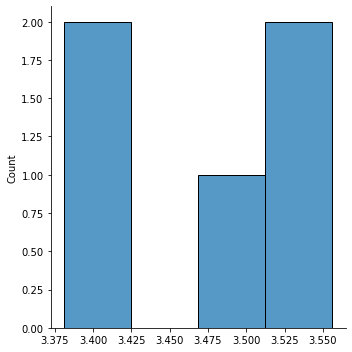
\includegraphics[width=8cm, height=7cm]{gpa_histo1.5}
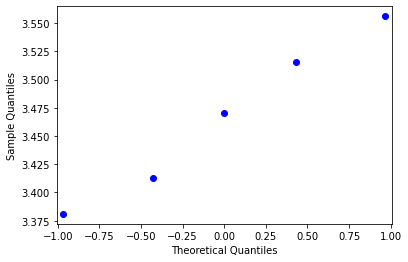
\includegraphics[width=8cm, height=7cm]{gpa_qq1.5}

Gráfico Distribución de Varianza para GPA y QQ Plot (5 muestras)\\
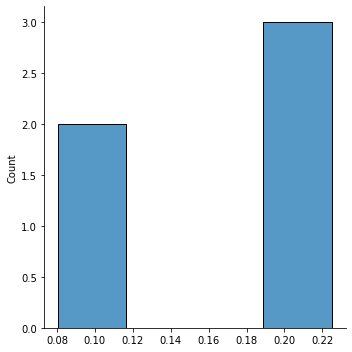
\includegraphics[width=8cm, height=7cm]{gpa_histo2.5}
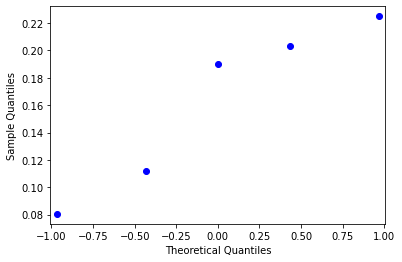
\includegraphics[width=8cm, height=7cm]{gpa_qq2.5}
\clearpage
Gráfico Distribución de Media para Horas de Estudio Semanasy QQ Plot (5 muestras)\\
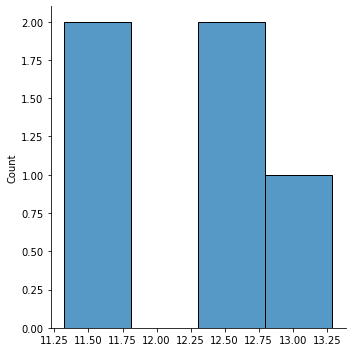
\includegraphics[width=8cm, height=7cm]{horas_histo1.5}
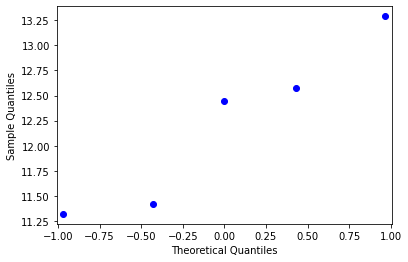
\includegraphics[width=8cm, height=7cm]{horas_qq1.5}

Gráfico Distribución de Varianza para Horas de Estudio Semanasy QQ Plot (5 muestras)\\
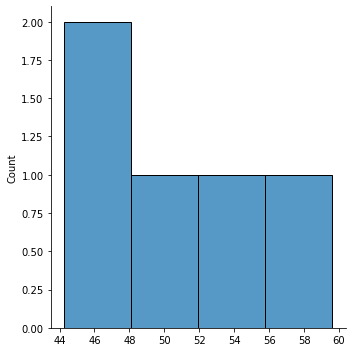
\includegraphics[width=8cm, height=7cm]{horas_histo2.5}
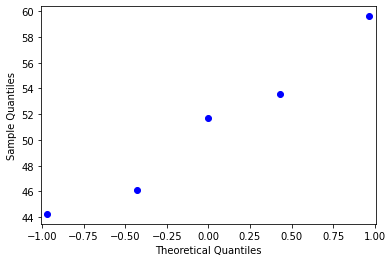
\includegraphics[width=8cm, height=7cm]{horas_qq2.5}

Continuando con el experimento hemos obtenido una tabla mostrando la media y desviación estándar de cada muestra, la diferencia de estas con la media y desviación estándar de la población que previamente habíamos calculado en la sección 1. \\

Asumiendo que la media de cada muestra es un estimador de la media poblacional se ha encontrado el error estándar del estimador de la media poblacional dando como resultado una media de error estándar de 0.05785757152145068 para el GPA y de 0.9842321350674442
para las horas de estudio semanales.\\

Finalmente hemos obtenido una nueva variable cuantitativa de nuestra encuesta la cual fue la edad de los estudiantes encuestados y hemos obtenido que las edades de se distribuyen de forma exponencial tal como se muestra en la gráfica a continuación. La primera gráfica muestra una simulación de distribución exponencial mientras que la segunda gráfica es la distribución de las edades de los estudiantes.\\

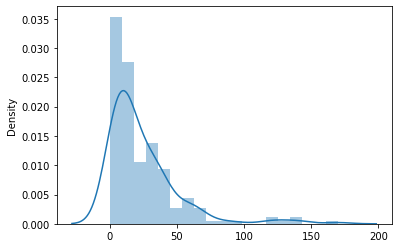
\includegraphics[width=8cm, height=7cm]{dist1}
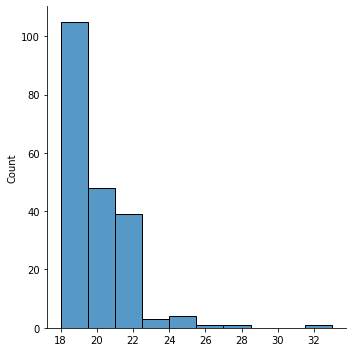
\includegraphics[width=8cm, height=7cm]{dist2}

Asi mismo hemos obtenido que el valor del parámetro poblacional a partir de el método de máxima verosimilitud es de teta igual a 17.99.

\clearpage
\end{document}
